% The infinite binary tree 2^{<ω} of finite binary strings, extended downward.
% Source: book/tex/set-theory/forcing.tex (§ Separative posets, infinite binary tree).
\documentclass[border=2mm]{standalone}
\usepackage{tikz}
\usepackage{amssymb}
\begin{document}
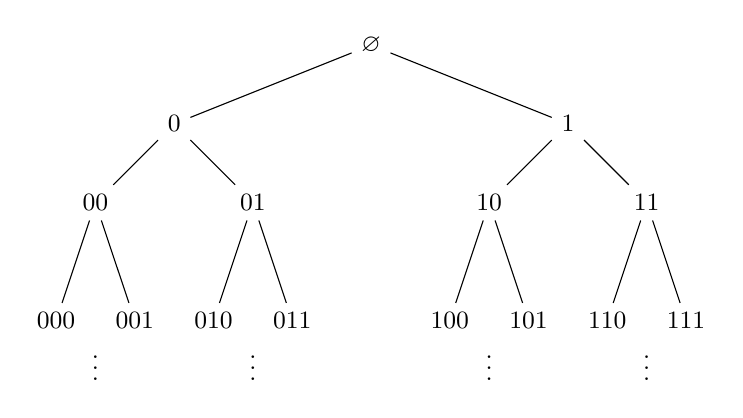
\begin{tikzpicture}[scale=0.5, every node/.style={font=\small}]
  \node (P) at (0,4) {$\varnothing$};
  \node (P0) at (-5,2) {$0$};   \node (P1) at (5,2) {$1$};
  \node (P00) at (-7,0) {$00$}; \node (P01) at (-3,0) {$01$};
  \node (P10) at (3,0) {$10$};  \node (P11) at (7,0) {$11$};
  \node (P000) at (-8,-3) {$000$}; \node (P001) at (-6,-3) {$001$};
  \node (P010) at (-4,-3) {$010$}; \node (P011) at (-2,-3) {$011$};
  \node (P100) at (2,-3) {$100$};  \node (P101) at (4,-3) {$101$};
  \node (P110) at (6,-3) {$110$};  \node (P111) at (8,-3) {$111$};
  \draw (P0) -- (P) -- (P1);
  \draw (P00) -- (P0) -- (P01);
  \draw (P10) -- (P1) -- (P11);
  \draw (P000) -- (P00) -- (P001);
  \draw (P010) -- (P01) -- (P011);
  \draw (P100) -- (P10) -- (P101);
  \draw (P110) -- (P11) -- (P111);
  \node at (-7,-4) {$\vdots$}; \node at (-3,-4) {$\vdots$};
  \node at (3,-4) {$\vdots$};  \node at (7,-4) {$\vdots$};
\end{tikzpicture}
\end{document}
